\section{Extending the Game Code} \label{section: git}
We extended the code by creating a crafting recipe for a cake. The recipe involves 3 milk buckets, 3 wheat, 2 sugar and 1 egg. Upon crafting the cake the player gets a cake and 3 empty buckets. The cake recipe in JavaCraft is the same cake recipe in Minecraft.
In order to be able to craft a cake, we have added the following blocks:
\begin{enumerate}
    \item Cow
    \item Chicken
    \item Wheat
    \item Sugar Cane
\end{enumerate}

The world generation has been modified to include the four aforementioned blocks. In particular, the method \texttt{generateWorld} has been modified.

\begin{lstlisting}
public static void generateWorld() {
    Random rand = new Random();
    for (int y = 0; y < worldHeight; y++) {
      for (int x = 0; x < worldWidth; x++) {
        int randValue = rand.nextInt(100);
        if (randValue < 10) {
          world[x][y] = WOOD;
        } else if (randValue < 20) {
          world[x][y] = LEAVES;
        } else if (randValue < 28) {
          world[x][y] = WHEAT;
        } else if (randValue < 37) {
          world[x][y] = CHICKEN;
        } else if (randValue < 45) {
          world[x][y] = STONE;
        } else if (randValue < 60) {
          world[x][y] = IRON_ORE;
        } else if (randValue < 65) {
          world[x][y] = COW;
        } else if (randValue < 70) {
          world[x][y] = SUGARCANE;
        } else {
          world[x][y] = AIR;
        }
      }
    }
}
\end{lstlisting}

In addition, we have implemented new items:

\begin{enumerate}
    \item Milk Bucket
    \item Egg
    \item Empty Bucket
    \item Sugar
    \item Cake
\end{enumerate}

The recipes for the aforementioned items (except for the milk bucket and egg) each have their own methods: \texttt{craftBucket}, \texttt{craftCake}, and \texttt{craftSugar}. Their methods are as follows:

\begin{lstlisting}
public static void craftBucket() {
    if (craftedItemsContains(CRAFTED_IRON_INGOT, 3)) { 
      removeItemsFromCraftedItems(CRAFTED_IRON_INGOT, 3);
      addCraftedItem(CRAFTED_BUCKET);
      System.out.println("Crafted Bucket.");
    } else {
      System.out.println("Insufficient resources to craft Bucket.");
    }
}
public static void craftCake() {
    boolean cond = craftedItemsContains(CRAFTED_SUGAR, 2) && inventoryContains(EGG, 1) && inventoryContains(WHEAT, 3) && inventoryContains(MILK_BUCKET, 3);
    if (cond) {
      removeItemsFromCraftedItems(CRAFTED_SUGAR, 2);
      removeItemsFromInventory(EGG, 1);
      removeItemsFromInventory(WHEAT, 3);
      removeItemsFromInventory(MILK_BUCKET, 3);
      addCraftedItem(CRAFTED_BUCKET);
      addCraftedItem(CRAFTED_BUCKET);
      addCraftedItem(CRAFTED_BUCKET);
      addCraftedItem(CRAFTED_CAKE);
      System.out.println("Crafted Cake.");
    } else {
      System.out.println("Insufficient resources to craft Cake.");
    }
}
public static void craftSugar() {
    if (inventoryContains(SUGARCANE, 1)) {
      removeItemsFromInventory(SUGARCANE, 1);
      addCraftedItem(CRAFTED_SUGAR);
      System.out.println("Crafted Sugar.");
    } else {
      System.out.println("Insufficient resources to craft Sugar.");
    }
}
\end{lstlisting}

Note that we call for the methods \texttt{craftedItemsContains} and \texttt{removeItemsFromCraftedItems}, which were not in the original code. This is done because items such as the iron bucket and sugar are stored in \texttt{craftedItems}, which is separate from the inventory \texttt{inventory}. The method is similar to the existing methods \texttt{inventoryContains} and \texttt{removeItemsFromInventory} with the only difference being which inventory the method accesses. The methods \texttt{craftedItemsContains} and \texttt{removeItemsFromCraftedItems} are as follows:

\begin{lstlisting}
    public static boolean craftedItemsContains(int item) {
    return craftedItems.contains(item);
  }
    public static boolean craftedItemsContains(int item, int count) {
    int itemCount = 0;
    for (int i : craftedItems) {
      if (i == item) {
        itemCount++;
        if (itemCount == count) {
          return true;
        }
      }
    }
    return false;
  }
  public static void removeItemsFromCraftedItems(int item, int count) {
    int removedCount = 0;
    Iterator<Integer> iterator = craftedItems.iterator();
    while (iterator.hasNext()) {
      int i = iterator.next();
      if (i == item) {
        iterator.remove();
        removedCount++;
        if (removedCount == count) {
          break;
        }
      }
    }
  }
\end{lstlisting}

The Milk Bucket can be obtained if the player interacts with a cow while the player has at least one bucket in their inventory. The Egg can be obtained when interacting with the chicken. Both the cow and the chicken cannot be mined as it does not make much sense to mine an animal. Upon trying to mine either animal, the message \texttt{Why would you want to mine an animal? D:} appears. For this to work the method \texttt{mineBlock} has been modified.

\begin{lstlisting}
    public static void mineBlock() {
    int blockType = world[playerX][playerY];
    if (blockType != AIR && blockType != COW && blockType != CHICKEN) {
      inventory.add(blockType);
      world[playerX][playerY] = AIR;
      System.out.println("Mined " + getBlockName(blockType) + ".");
    } else if (blockType == AIR) {
      System.out.println("Cannot mine air.");
    } else {
      System.out.println("Why would you want to mine an animal? D:");
    }
    waitForEnter();
  }
\end{lstlisting}

The flowchart on how to craft a cake can be found below:

{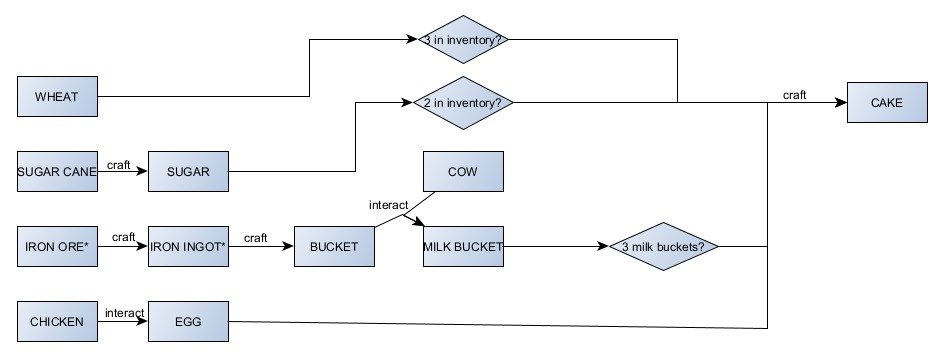
\includegraphics[width=\textwidth]{../flowchart/cake.jpg}}
